\chapter{Testovací program}
Testovací systém běžící na serveru testovací laboratoře se skládá z několika samostatných částí. Základem celého systému je databáze uchovávající všechny informace o struktuře testovací laboratoře, informace o všech modelech testovaných zařízení a data s výsledky jednotlivých testů. Další součástí je program testlab, jenž se stará o celý průběh testování. Několika málo přepínači lze nastavit průběh testování. Další součástí je sada programů nazývající se testovací API, tyto programy slouží k usnadnění psaní jednotlivých testů. Nedílnou součástí testovacího systému jsou testovací skripty, které lze rozdělit na skripty pro stáhnutí projektu, kompilaci platforem, testování zařízení a úklid projektu. Tyto testovací skripty odpovídají testovacím procedurám postupu testování založeného na modelech popsaného v předchozí kapitole. Poslední součástí testovacího systému je webový interface pro sledování výsledků testování a nastavování chování testovacího systému.

\section{Adresářová struktura testovacího systému}

Jednotlivé částí testovacího systému jsou rozloženy v adresářové struktuře serveru následovně. Všechny součásti testovacího programu testlab jou umístěny v adresáři /opt/testlab/main a všechny programy testovacího API jsou umístěny v adresáři /opt/testlab/api. Obě zmíněné cesty jsou přidány do systémové proměnné PATH, aby bylo možné programy spouštět odkudkoli. Sdílené knihovny, které využívá testovací program a programy testovacího API jsou umístěny v adresáři /opt/testlab/lib. Jelikož sdílené knihovny používá pouze program testlab, hlavičkové soubory nejsou na server umisťovány. Popsané tři adresáře tvořící první část testovacího systému se za běhu nemění a zůstává stejná. Jedinou výjimkou je aktualizace testovacího systému, při které mohou být opraveny chyby, či může být přidán nový program do testovacího API. Aktualizaci testovacího programu provádí pouze administrátor testovacího systému.

Druhá část adresářové struktury testovacího systému obsahuje soubory a adresáře měnící se v průběhu běhu testovacího systému. Tato část se nechází v adresáři /var/testlab a je rozdělena na následující adresáře. Prvním adresářem je clean obsahující skripty pro zajištění úklidu po překladu jednotlivých platforem. Adresář compile obsahuje skripty zajišťující kompilaci jednotlivých výrobků všech platforem každého projektu. Pro každý projekt je v tomto adresáři sada skriptů, platforma a produkt se zadává jako parametr. V adresáři checkout nalezneme skripty starající se o  stáhnutí či aktualizaci zdrojových kódu každého projektu. Pro stahování zdrojových kódů se budou často využívat repozitáře a konkrétně bude využit verzovací systém git. Adresář source slouží k uchování zdrojových kódu jednotlivých projektů. Project je pracovním adresářem kam jsou kopírovány zdrojové kódy jednotlivých platforem a kde jsou následně překládány. Dále je tento adresář rozdělen do jednotlivých podadresářů dle jednotlivých releasů překládaného firmwaru. V každém adresáři releasu jsou adresáře pro každou testovanou platformu. Adresáře jednotlivých releasu se před ukončení kompilace odstraňují, jelikož dále nejsou potřeba a zabírají velký prostor na disku. Přeložený firmware všech výrobků je ukládán do adresáře firmware a do podadresáře s názevem identifikačního čísla releasu, pro který byl firmware přeložen. Tento adresář bude později přesunut na jiný disk vzhledem k omezené kapacitě ssd disku. Testovací skripty se nacházejí v adresáři tests. Adresář tests se dále dělí na podadresáře s názvy funkcí. V adresářích s názvem funkcí se nacházejí jednotlivé testovací skripty jejichž název je shodný s testovací procedurou. Posledním adresářem této části testovacího systému je adresář logs. V adresáři logs se ukládají logy z jednotlivých fází testování. Ukládájí se zde logy ze stáhování zdrojových kódů, ze samotné kompilace všech výrobků a z úklidu po překladu. Adresář je členěn podle typu logu a dále podle releasu testovaného firmwaru. Adresář s logy bude postupně přesunut na jiný disk obdobně jako adresář firmware. Chybové logy z prováděných testů se ukládají do databáze.

\begin{figure}[h]
  \centering
  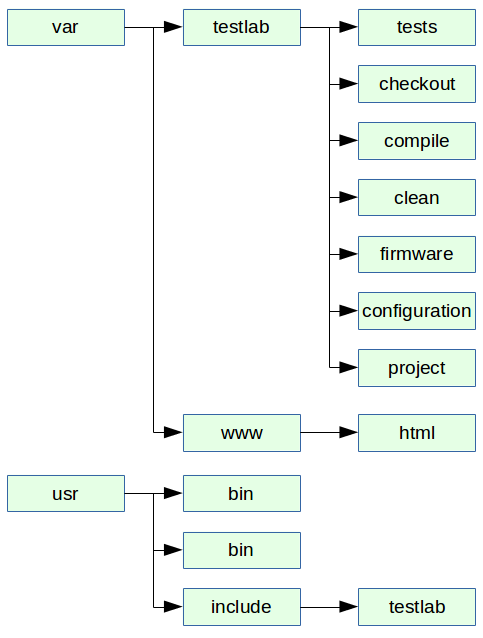
\includegraphics[width=.4\LW]{adresar_struktura}
  \caption{Adresářová struktura testovacího systému}
  \label{fig:adresar_struktura}
\end{figure}

Třetí část testovacího systému se nachází v adresáři /var/www/html. Tuto část testovacího systému tvoří webové stránky testovacího systému

\section{Struktura databáze}
Jak již bylo dříve zmíněno všechny informace o testovaných zařízeních a výsleddcích testů jsou uloženy v databázi. K těmto účelům byla využita MySQL databáze. K databázi má přístup samotný testovací program testlab, všechny programy testovacího api a v neposlední řadě webová aplikace sloužící k administraci modelů testovaných zařízení a reportování výsledků testů. Pro organizované uchovávání všech dat byla navržena základní struktura databáze, která se časem s přibývající funkcionalitou testovacího systému může rozšiřovat. Jednotlivé tabulky této struktury jsou popsány v samostatných sekcích.

\subsection{Tabulka fwrelease}
První a základní tabulkou celého systému je fwreleases. V tabulce fwreleases jsou uloženy informace o testovaném releasu. Release je vytvořen a uložen do databáze při každém spuštění programu testlab, aby bylo možné rozlišit jednotlivá testování. Všechny tabulky, které uchovávají informace o konkrétním testu odkazují právě na jeden konkrétní záznam této tabulky. Tabulka fwreleases prozatím obsahuje pouze 3 údaje. Položka idfwreleases je primárním klíčem tabulky, položka date uchovává datum a čas vzniknu releasu a položka type určije o jaký typ vydání firmwaru se jedná.

\begin{figure}[h]
  \centering
  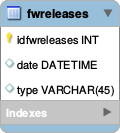
\includegraphics[scale=0.6]{database_fwreleases}
  \caption{Tabulka fwreleases}
  \label{fig:database_fwreleases}
\end{figure}

\subsection{Tabulka platforms}
Tabulka platforms obsahuje informace o jednotlivých platformách. Platforma je skupina výrobků postavena na společných zdrojových kódech a na jednom procesoru. Platformy se dále dělí na výrobky. Tabulka obsahuje prozatím následující 4 položky. Položka idplatforms, která je primárním klíčem tabulky, položka name slouží k uložení názvu tabulky, dále položky timeout\_checkout a timeout\_build sloužící k nastavení timeoutu skriptu pro stažení zdrojových kódu platfromy a pro přeložení zfrojových kódů platformy.

\begin{figure}[h]
  \centering
  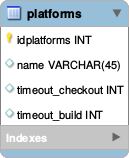
\includegraphics[scale=0.6]{database_platforms}
  \caption{Tabulka platforms}
  \label{fig:database_platforms}
\end{figure}

\subsection{Tabulka products}
Tabulka products obsahuje informace o jednotlivých produktech. V této tabulce nejsou produkty chápány jako jednotlivé produkty v testovací laboratoři, ale pouze jednotlivé druhy firmwaru. Rozdělení bylo provedeno z důvodu možnosti nahrání stejného firmwaru do různého hardwaru a tím vzniknutím nového výrobku. Tabulka products obsahuje pouze 3 následující položky. Položka idproducts, které je primárním klíčem tabulky, položka idplatforms odkazující na danou platformu v tabulce platforms. Poslední položka name definuje název produktu.

\begin{figure}[h]
  \centering
  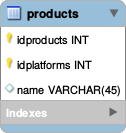
\includegraphics[scale=0.6]{database_products}
  \caption{Tabulka products}
  \label{fig:database_products}
\end{figure}

\subsection{Tabulka checkout}
Tabulka checkout slouží pro ukládání výsledků stažení zdrojových kódů z repozitáře. Tabulka obsahuje 4 položky. Položka idcheckout je primárním klíčem tabulky. Položka idplatforms odkazuje na tabulku platforms a udává o jaké zdrojové kódy platformy se jedná. Položka idfwreleases odkazuje na tabulku fwreleases a udává k jakému testování výsledek odpovídá. Poslední položka state ukládá stav výsledku skriptu pro stažení aktuálních zdrojových kódů platformy.

\begin{figure}[h]
  \centering
  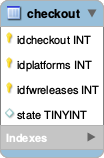
\includegraphics[scale=0.6]{database_checkout}
  \caption{Tabulka checkout}
  \label{fig:database_checkout}
\end{figure}

\subsection{Tabulka builds platform}
Tabulka builds\_platform slouží k ukládání výsledků překladu celé platformy, čili všech výrobků dané platformy. Tabulka obsahuje celkem 4 položky. Položka idbuilds\_platform je primárním klíčem tabulky. Položka idplatforms odkazuje na tabulku platforms a udává platformy, které se výsledek překladu týká. Položka idfwreleases odkazuje na tabulku fwreleases a udává k jakému vydání firmwaru je zdrojový kód překládán. Poslední položka state představuje stav ukončení překladu firmwaru celé platformy.

\begin{figure}[h]
  \centering
  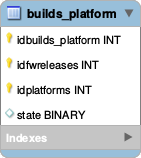
\includegraphics[scale=0.6]{database_buildsplatform}
  \caption{Tabulka builds platform}
  \label{fig:database_buildsplatform}
\end{figure}

\subsection{Tabulka build product}
Tabulka builds\_product slouží k ukládání výsledků překladu jednotlivých výrobků. Tabulka obsahuje celkem 4 položky. Položka idbuilds\_product je primárním klíčem tabulky. Položka idproducts odkazuje na tabulku products a udává jakého produktu se výsledek překladu týká. Položka idfwreleases odkazuje na tabulku fwreleases a udává k jakému vydání firmwaru je zdrojový kód překládán. Poslední položka state představuje stav ukončení překladu firmwaru daného produktu.

\begin{figure}[h]
  \centering
  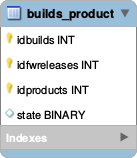
\includegraphics[scale=0.6]{database_buildsproduct}
  \caption{Tabulka builds product}
  \label{fig:database_buildsproduct}
\end{figure}

\subsection{Tabulka routers}
Tabulka routers je určena pro uložení modelů všech routerů přítomných v testovací laboratoři. Položky v této tabulce tedy nepředstavují již dříve zmíněný produkt, ale skutečný testovaný výrobek. Každá položka této tabulky představuje jeden model testovaného zařízení, tudíž testovány jsou pouze routery které jsou uloženy v této tabulce. Kompletní model zařízení netvoří pouze tabulka routers. Model zařízení tvoří i další tabulky, které jsou s tabulkou routers provázány různými typy vazeb. Tabulka routers obsahuje následující položky. Položka idrouters je primárním klíčem tabulky. Položka idproducts odkazuje do tabulky products a definuje jaký firmware má být nahrán do tohoto výrobku. Položka idplatform odkazuje do tabulky platforms a definuje platformu na které je daný výrobek postaven. Další položka name slouží k pojmenování výrobku v testovací laboratoři, tato položka slouží pouze k snadnému rozeznání výrobků v testovací laboratoři. Položka port definuje v jakém portu switche je zapojen primární ethernet testovaného výrobku. Výchozí IP adresu  primárního portu testovaného zařízení definuje položka address. Prozatím poslední položkou tabulky routers je protocol. Položka protocol určuje primární protocol pomocí kterého testovaný výrobek komunikuje s testovací aplikací.

\begin{figure}[h]
  \centering
  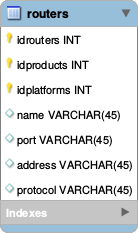
\includegraphics[scale=0.6]{database_routers}
  \caption{Tabulka routers}
  \label{fig:database_routers}
\end{figure}

\subsection{Tabulka functions}
Další tabulkou pomocí níž se tvoří model testovaného zařízení je tabulka functions. Tabulka functions sdružuje data o jednotlivých funkcích, které mohou testované výrobky podporovat. Tabulka obsahuje následující položky definující informace o dané funkci. Položka idfunctions je primárním klíčem tabulky. Položka name definuje název pod kterým je daná funkcionalita reprezentována v testovacím systému. Poslední je položka order určující pořadí v jakém mají být funkcionality testovány.

\begin{figure}[h]
  \centering
  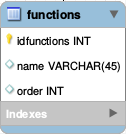
\includegraphics[scale=0.6]{database_functions}
  \caption{Tabulka functions}
  \label{fig:database_functions}
\end{figure}

\subsection{Tabulka dependences}
Třetí tabulkou tvořící model testovaného zařízení je tabulka dependences. Pomocí tabulky dependences je možné definovat závisloti jednotlivých funkcí na jiných, tudíž je možné definovat spuštění jednoho testu v závislosti na výsledku jednoho nebo více předešlých testů. Popsaná funkcionalita je realizována pomocí následujících třech položek. Položka target odkazuje na určitou funkci a určuje funkci, která je závislá na výsledku jiných funkcí. Položka dependences dále odkazuje na zdrojovou funkci a určuje na výsledku jaké funkce závisý provedění testů funkce target. Poslední položka určuje typ závislosti. Podporovány jsou dva typy závislosti, buď musí být správně otestovány všechny předešlé funkce nebo stačí úspěšný výsledek testů pouze jedné ze zdrojových funkcí.

\begin{figure}[h]
  \centering
  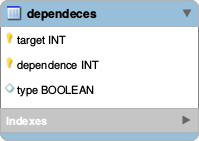
\includegraphics[scale=0.6]{database_dependences}
  \caption{Tabulka dependences}
  \label{fig:database_dependences}
\end{figure}

\subsection{Tabulka routers has functions}
Další tabulkou tvořící model testovaného zařízení je tabulka routers\_has\_functions. Pomocí této tabulky jsou každému modelu přiřazeny funkce, které je možné testovat. Přiřazení je realizováno pomocí dvou cizích klíčů odkazujících do tabulek routers a functions. Do tabulky routers odkazuje položka idrouters a položka idfunctions odkazuje do tabulky functions.

\begin{figure}[h]
  \centering
  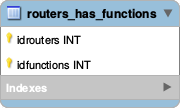
\includegraphics[scale=0.6]{databse_routershasfunctions}
  \caption{Tabulka routers has functions}
  \label{fig:databse_routershasfunctions}
\end{figure}

\subsection{Tabulka procedures}
Tabulka procedures již neslouží k uchování dat z abstraktního pohledu testování založeného na modelech. Tabulka uchovává jednotlivé spustitelné procedury sloužící k testování funkcí. Procedury jsou definované následujícímy položkami. Položka idprocedures je primárním klíčem tabulky. Položka idfunctions odkazuje na záznam v tabulce functions a definuje funkci kterou má procedura testovat. Položka name definuje název procedury pod kterým se spustitelný skript v testovacím systému reprezentuje. Položka unit slouží k lepší reprezentaci výsledné hodnoty daného skriptu. Pokud procedura vrací hodnotu která je definována jakoukoliv jednotkou, může být v položce unit tato jednotka definována. Položka timeout určuje čas maximálního běhu testovací procedury, po uplynutí tohoto času je testovací procedura ukončena.

\begin{figure}[h]
  \centering
  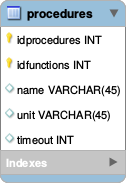
\includegraphics[scale=0.6]{database_procedures}
  \caption{Tabulka procedures}
  \label{fig:database_procedures}
\end{figure}

\subsection{Tabulka tests router}
Výsledky testování jsou ukládány do tří různých tabulek pro jednodušší reportování výsledků testování. První tabulkou je tests\_router do níž jsou ukládány informace o testování celého zařízení. Za úspěšný se tento test považuje pokud všechny procedury spustěné na testovaném zařízení byly ukončeny úspěšně. Tabulka obsahuje 4 následující položky. Položka idtests\_router je primárním klíčem tabulky. Položka idrouters odkazuje na tabulku routers a určuje jakému zařízení je výsledek testu určen. Položka idfwreleases odkazuje na tabulku fwreleases a určuje k jakému vydání firmwaru je výsledek testu přiřazen. Poslední položkou je samotný výsledek testu a to položka result.

\begin{figure}[h]
  \centering
  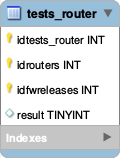
\includegraphics[scale=0.6]{database_testsrouter}
  \caption{Tabulka tests router}
  \label{fig:database_testsrouter}
\end{figure}

\subsection{Tabulka tests function}
Druhou tabulkou sloužící k ukládání výsledků testů je tabulka tests\_function. Tato tabulka sdružuje výsledky všech testovacíh procedur dané funkce na jednom testovaném zařízení. Test funkce je považován za úspěšný, jestliže všechny testoavné procedury této funkce proběhli úspěšně. Tabulka tests\_function obshauje pět následujících položek. Položka idtests\_function je primárním klíčem tabulky. Položka idfunctions odkazuje na tabulku functions a definuje o jakou testovanou funkci se jedná. Položka idfwreleases odkazuje na tabulku fwreleases a definuje k jakému testovanému firmwaru je výsledek testování funkce přiřazen. Položka idrouters odkazuje na tabulku routers a definuje jakému zařízení je výsledek testu přiřazen. Poslední položka result určuje samotný výsledek testu.

\begin{figure}[h]
  \centering
  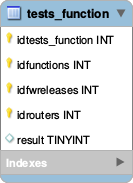
\includegraphics[scale=0.6]{database_testsfunction}
  \caption{Tabulka tests function}
  \label{fig:database_testsfunction}
\end{figure}

\subsection{Tabulka tests procedure}
Poslední tabulkou sloužící k ukládání výsledků testů je tabulka tests\_procedures.V této tabulce jsou uloženy vyýsledky ze všech spuštěných testovacích procedur. K identifikaci výsledku testu z každé testovací procedury slouží šest následujících položek. Položka idtests\_procedure je primárním klíčem tabulky. Položka idprocedures odkazuje na tabulku procedures a definuje jaké testovací procedury se výsledek týká. Položka idrouters odkazuje na tabulku routers a definuje jakému testovanému zařízení má být výsledek přiřazen. Položka idfwreleses odkazuje na tabulku fwreleases a definuje jakému testovanému releasu má být výsledek testu přiřazen. Položka result určuje výsledk testu. Poslední položka value slouží k uložení jakékoliv pomocné informační hodnoty, kterou může vygenerovat testovací skript.

\begin{figure}[h]
  \centering
  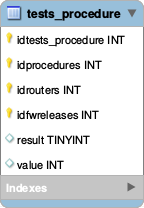
\includegraphics[scale=0.6]{database_testsprocedure}
  \caption{Tabulka tests procedure}
  \label{fig:database_testsprocedure}
\end{figure}

\subsection{Tabulka logs}
Tabulka logs schromažďuje všechny chybové výpisy, jenž jsou vygenerovány testovacímy skripty. Tabulka obsahuje pět následujících položek. Položka idlogs je primárním klíčemm tabulky. Položka idprocedures odkazje na tabulku procedures a definuje k jaké testovací proceduře je chybová hláška přiřazena. Položka idrouters odkazuje na tabulku routers a definuje na jakém testovaném zařízení chybová hláška vznikla. Položka idfwreleases odkazuje na tabulka fwreleases a definuje jakého firmwaru se chybová hláška týká. Poslední položka event určuje samotný text chybové hlášky.

\begin{figure}[h]
  \centering
  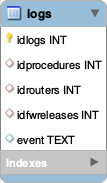
\includegraphics[scale=0.6]{database_logs}
  \caption{Tabulka logs}
  \label{fig:database_logs}
\end{figure}

\section{Popis programu}

O průběh celého testu se stará program testlab. Testlab je program psaný v jazyc C. Program po spuštění otevře systémový log pro možnost logování chyb do systémového logu. Filtrováný systémový log by měl později být zobrazován na webowém rozhraní testovacího systému. První hláškou do systémového logu je informace o spuštění programu testlab, daným uživatelem a v určený čas. Po otevření systémového logu program rozebírá parametry na příkazové řádce. Parametry jsou rozebíráný pomocí funkce getopts. Pomocí parametrů lze ovlivnit chování programu testlab.

Jediným poviným parametrem je název testovaného projektu v daném repozitáři. Před tento povinný parametr je možné umístit dva volitelné přepínače upravující chování programu. Přepínač -r určuje zda přeložený firmware bude označen jako release nebo beta verze, jestliže parametr není zadán firmware je přeložen jako beta verze. Druhým přepínačem -b s povinným parametrem určíme větev repozitáře ze které mají být zdrojové kódy kompilovány.

\begin{figure}[h]
  \centering
  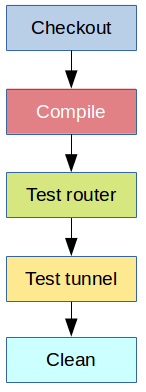
\includegraphics[width=.2\LW]{program_schema}
  \caption{Základní schéma testovacího programu}
  \label{fig:program_schema}
\end{figure}

Po rozebrání parametrů se provádějí přípravné kroky pro samotné testování. V prvním kroku je vytvořen nový release firmwaru a následně vložen do databáze. V adresáři project je vytvořen nový adresář s názvem identifikačního čísla testovaného releasu. Po těchto krocích je založen nový release firmwaru a může se přejít k samotnému testování.

\subsection{Checkout}
V prvním kroku testování jsou stahovány zdrojové kódy testovaného projektu. Projekt je předán programu jako parametr a detailní informace o projektu jsou získány z databáze. Po získání všech informací je spuštěn program checkout  a v hlavním programu se pouze čeká na ukončení programu checkout.

Program checkout je spouštěn se třemi parametry. Prvním parametrem je identifikační číslo testovaného releasu, druhým parametrem je identifikační číslo stahovaného projektu a posledním parametrem je název stahovaného projektu. Nejdříve je kontrolováno jestli existuje skript provádějící stažení platformy. Stahování zdrojových kódů pomocí skriptu bylo zavedo z důvodu komplexnosti této operace. Jedním ze složitějších případů checkout skriptu může být stahování zdrojových kódů platformy ze dvou a více různých repozitářů. Po zkontrolování existence skriptu je checkout skript spuštěn. Chzbový i standardní výstup skriptu je přesměrován do souboru s logem. Tento soubor se nachází v adresáři logs, dále v podadresáři s názvem identifikačního čísla releasu, kde jsou samotné soubory pojmenované podle názvu stahovaného projektu. U skriptu je dále kontrolované jestli čas spuštění nepřekračuje nastavený timeout. V případě překročení času spuštění je skript ukončen s chybovým návratovým kódem. Na závěr je výsledek stažení projektu uložen do databáze. V této fázi testování je také zjišťována verze firmwaru a hash posledního commitu zdrojového kódu.

Po ukončení aktualizace zdrojových kódů projektu jsou zdrojové kódy kopírovány do pracovních adresářu jednotlivých platforem. V těchto pracovních adresářích jsou zdrojové kódy dále kompilovány.

\subsection{Compile}
Další fází každého testování je kompilace zdrojových kódů všech platforem. Pro ukládání přeložených firmwarů je vytvořen adresář s názvem identifikačního čísla releasu v adresáří firmware. Po vytvoření tohoto adresáře je pro každou platformu spuštěn program compile. V programu testlab se dále čeká na ukončení všech programů compile.

Program compile je spuštěn se třemi parametry. Prvním parametrem je identifikační číslo testovaného releasu, druhým parametrem je identifikační číslo překládané platformy a posledním parametrem je název překládané platformy. Program compile nejdříve provede změnu pracovního adresáře na adresář se zdrojovými kódy překládané platformy. Program dále z databáze získá názvy všech produktů patřících pod zpracovávanou platformu. Nyní je provedena kontrola existence skriptu provádějícího samotnou kompilaci zdrojových kódů platformy. Jednotlivé produkty se spouštěnému skriptu předávají jako parametr. V případě existence skriptu pro kompilaci zpracovávané platformy je postupně tento skript spouštěn s parametry všech výrobků. Standardní a chybový výstup spuštěného skriptu je přesměrováván do souboru obdobně jako u programu checkout. Díky uložení všech výstupů jsou informace o překladu firmwarů zpětně dostupné. Doba běhu skriptu je kontrolována a jestliže přesáhne zadaný timeout, skript je předčasně ukončen s chybovým návratovým kódem. Toto opatření je prováděno z důvodu předejití zaseknutí celého testovacího systému. Každý přeložený firmware je zkopírován z adresáře kde byl přeložen do adresáře určeného pro přeložené firmwary aktuálního releasu. Po zkopírování firmwaru je výsledek překladu každého výrobku uložen do databáze. Výsledek přeložení platformy, čili všech výrobků je na závěr této sekce taktéž uložen do databáze, z důvodu snadnější prezentace dat.

\subsection{Remote server}
Po ukončení překladu všech výrobků končí fáze kontinuální integrace a začíná systémové testování na konkrétním hardwaru. Pro účely testování se s každým routerem udržuje pernamentní spojení pomocí jednoho z protokolů telnet nebo ssh. Způsob komunikace pomocí pernamentního spojení bylo zvoleno jelikož díky velmi častému opětovnému připojování, zařízení již dále nepříjmala další žádosti o připojení. Nejdříve jsou z databáze vybrány všechny testované zařízení a pro každé testované zařízení je spuštěn program remote server udržující pernamentní spojení.

Program remote server je spouštěn se třemi povinnými parametry. Prvním parametrem je identifikátor zařízení. Identifikátor zařízení je číslo pomocí kterého mohou testovací aplikace komunikovat s zařízením. V rámci testovacího systému je v tomto parametru předáváno identifikační číslo zařízení použité v databázi. Druhým parametrem je IP adresa zařízení se kterým má být udržováno spojení. Posledním povinným parametrem je protokol kterým je prováděno spojení s zařízením. Nyní jsou podporovány dva protokoly a to telnet a ssh. Dále je možné použít volitelné parametry k úpravě defaultních přihlašovacích informací. Prvním voltelným parametrem lze změnit přihlašovací jméno do zařízení. Parametr lze změnit pomocí přepínače -u a defaultní hodnota je uživatel root. Dalším volitelný parametrem lze změnit přihlašovací heslo do zařízení. Parametr lze změnit pomocí přepínače -p a jeho defaultní hodnota je přihlašovací heslo root. Posledním volitelný parametrem je port na kterém se sestavuje spojení s testovaným zařízením. Port lze změnit pomocí přepínače -t a výchozí port se kterým se spojení navazuje je port 23.

\begin{figure}[h]
  \centering
  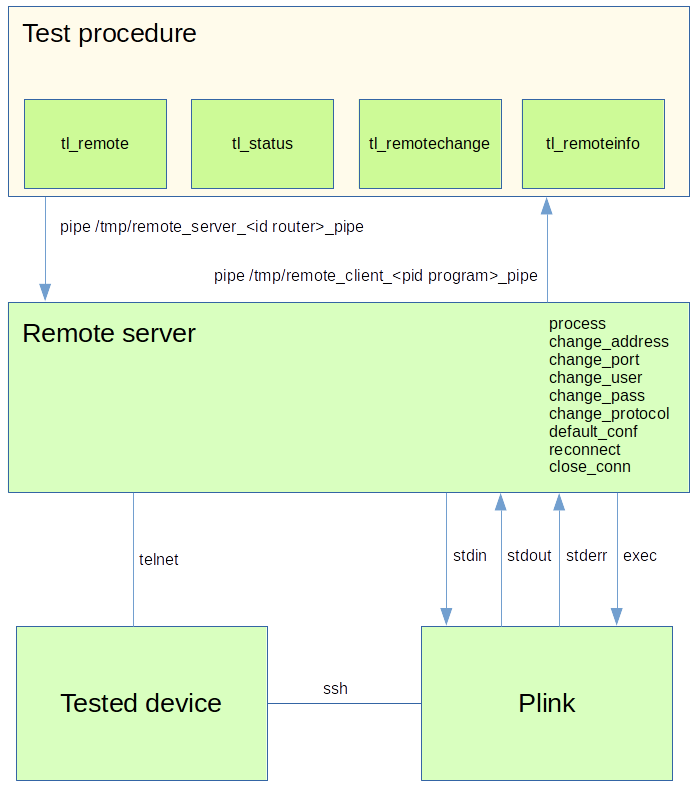
\includegraphics[width=.8\LW]{schema_remote}
  \caption{Schéma komunikace s testovaným výrobkem}
  \label{fig:schema_remote}
\end{figure}

Program remote server po zpracování všech parametrů vytvoří pojmenovanou rouru pomocí níchž bude komunikovat s programy testovacího API. Pojmenované roury jsou vytvářeny v adresáři /tmp. Název roury pomocí které server naslouchá příchozím požadavkům je remote\_server\_id\_pipe, kde id je identifikační číslo zařízení. Název roury pomocí které server předává odpověď dotazovanému programu je remote\_client\_pid\_pipe, kde pid je process id dotazovaného programu. Po vytvoření komunikační roury přichází fáze, kdy remote server čeká na příjem požadavku. Čekání na příjem požadavku je provedeno blokovaným otevřením čtecí pojmenované roury. Zde je program blokován až do otevření této roury nějakým klientským programem. Pokud nějaký program z testovacího API otevře tuto rouru a zapíše do ní data, remote server je přečte a uloží do datové struktury. Z datové struktury zprávy je zjištěno o jaký druh žádosti se jedná a žádost je provedena. Remote server podporuje následující typy žádosti.

\begin{itemize}
  \item Vykonaní příkazu
  \item Změna adresy připojení
  \item Změna portu připojení
  \item Změna přihlašovacího jména
  \item Změna přihlašovacího hesla
  \item Změna protokolu pro přihlášení
  \item Nastavení defaultní konfigurace
  \item Restart připojení do routeru
  \item Ukončení aplikace
  \item Informace o aktualní adrese
  \item Informace o aktualním portu
  \item Informace o aktualním uživateli
  \item Informace o aktualním hesle
  \item Informace o aktualním přihlašovacím protokolu
\end{itemize}

Po provedení příkazu remote server odpovídá jednou z těchto možných odpovědí.

\begin{itemize}
  \item Úspěšné vykonání
  \item Chyba ve skriptu
\end{itemize}

Funkce všech žádostí jsou zřejmě jasné z jejich názvů a tak dále bude detailně popsána hlavní a nejvíce používána žádost vykonání příkazu. Samotné vykonání příkazu je provedeno podle zvoleného protokolu.

\subsubsection{Telnet}
Při provedení příkazu pomocí protokolu telnet je nejdříve kontrolováno jestliže je spojení s testovaným zařízením aktivní. Jestliže spojení aktivní není, pokusí se program spojení s testovaným zařízením znovu navázat. V případě protokolu telnet byla napsána vlastní knihovna pro obsluhování telnet spojení. Navázání spojení je provedeno navázáním TCP spojení na portu, kde testované zařízení obsluhuje příchozí telnet spojení. Po navázání spojení jsou přijmatu parametry telnet relace a žádost o zadání přihlašovacího hesla. Nejdříve jsou zkontrolovány parametry relace a následně odeslána odpověď s parametry požadovaného chování telnet relace. Dále je odesláno přihlašovací jméno uživatele routeru. Po odeslání uživatelského jména je očekávána žádost o uživatelské heslo, které je také odesláno pomocí TCP spojení do zařízení. V případě úspěšného přihlášení, navazovací funkce vrací číslo file deskriptoru spojení. V případě jakéhokoliv neúspěchu při přihlášení do routeru je ukončeno TCP spojení s routerem.

Po úspěšném navázání spojení se mohou do routeru posílat příkazy, které by měl router vykonat. Samotné posílání příkazů do routeru je velice jednoduché. Příkaz je poslán pomocí vytvořeného TCP spojení do routeru a následně jsou příjmány data dokud není přijmuta sekvence znaků CR, LF, \# a mezera. Pro zamezení chyb při příjmu z routeru je nastaven timeout 60s. Po přečtení celé odpovědi z routeru je odpověď zpracována a pomocí pojmenované roury odeslána dotazovanému programu. Ukončení telnet spojení s testovaným zařízením je prováděno uzavřením daného TCP spojení.

\subsubsection{SSH}
Komunikace s testovaným zařízení skrz SSH protokol je řešeno pomocí programu Plink. Program Plink je z balíčku Putty-tools a vykonává funkci SSH klienta. Důvodem proč je použit program Pink místo standartního SSH klienta je možnost zadání přihlašovacího hesla jako parametr programu. Inicilaizace SSH spojení je tedy prováděna spuštěním programu Plink v novém procesu. Komunikace remote serveru s programem Plink probíhá pomocí standardního vstupu a výstupu. Před spuštěním programu Plink je standardní vstup a standardní výstup programu Plink připojen na nepojmenované roury vytvořené v programu remote server pro komunikaci s programem Plink. Po spuštění programu Plink je čten výstup programu Plink a je kontrolováno úspěšné navázání spojení s testovaným zařízením. V případě úspěšného spojení s testovaným zařízením inicializační funkce vrací PID programu plink. Pokud spojení nebylo úspěšně navázáno program Plink je ukončen a funkce vrací informaci o neúspěšném připojení.

Po úspěšném přihlášení je možné pomocí remote serveru skrz SSH protokolo posílat do testovaného zařízení příkazy. Při odesílání příkazů je nejdříve zkontrolováno sestavené spojení. Samotné odesílání příkazů je provedeno skrz nepojmenovanou rouru na standardní vstup aplikace Plink. Následně je čten standardní výstup aplikace Plink do příjmutí stejné sekvence znaků jako u telnet spojení. Z důvodu zamezení chyb při přenosu je pro příjem odpovědi nastaven timeout 60s. Pokud do vypršení timeoutu není příkaz zpracován spojení je uzavřeno a znovu inicializováno. Po příjmu celé odpvědi je odpověď zpracována a odeslána přes pojmenovanou rouru dotazovanému programu. Ukončení SSH spojení je prováděno posláním signálu kill programu Plink.

\subsection{Test}
Po úspěšném navázání spojení se všemi testovanémy zařízeními je započato samotné testování těchto zařízení. Testování bude rozděleno do několika sekcí podle typu provádění testů. V první fázi bude implementováno testování jednotlivých zařízení. Tento přístup testuje každý router samostatně a testování všech zařízení probíhá paralérně. V dalších fázích bude implementováno testování zařízení proti sobě, typickým testem může být spojení dvou zařízení IPsec tunelem. Třetím typem testování bude sekvenční testování zařízení, kdy při testování bude využit jedinečný zdroj, tudíž je nutné všechny zařízení testovat postupně.

Pro otestování všech zařízení je pro každé zařízení spuštěn program test se dvěma parametry. Prvním parametrem je identifikátor testovaného releasu. Druhým parametrem programu test je identifikační číslo testovaného zařízení. Po kontrole parametrů program test z databáze vybere všechny podporované funkce testovaného zařízení. Při zpracovávání každé funkce jsou z databáze vybrány všechny testovací procedury určené pro testování dané funkce. Nyní je vše připravené pro postupné spuštění všech testovacích procedur.

Před samotným spuštění je nejdříve kontrolována existence testovacího skriptu. Dále jsou vytvořeny nepojmenované roury pro předávání informací ze skriptu do testovacího programu. K předávání výsledné hodnoty testu je na rouru testovacího programu připojen standardní výstup spuštěného skriptu. Předávání chybových hlášek z testovaného skriptu je prováděno propojení chybového výstupu a nepojmenované roury testovacího programu. Po správném nastavení vstupů a výstupů je spuštěn testovací skript. Při běhu testovacího skriptu samotný program čeká jestli mu ze skriptu nepřicházejí nějaká data, či již nevypršel timeout pro provedení skriptu. Úspěšnost provedení testu je vyhodnocována z návratové hodnoty testovacího skriptu. Po ukončení skriptu je do databáze zapsán výsledek testu, hodnota testu předaná přes standardní výstup skriptu a chybové hlášky předané přes chybový výstup skriptu.

\subsection{Clean}
Nyní když jsou firmwary přeloženy a testy provedeny přichází fáze úklidu, kdy jsou ukončovány běžící programy a odstraňovány dočasné soubory. Nejdříve jsou ukončovány programy remote server udržující spojení s testovanými zařízeními. Ukončení programu je provedeno spuštěním programu remote exit, jenž pouze odesílá příslušnému remote server procesu komand ukončení aplikace. Po odlesání žádosti o ukončení všem programům remote server, hlavní program čeká na ukončení všech programů remote server a remote exit. V dalším kroku je provedeno odstranění všech přeložených platforem. Na každou platformu je zavolán program clear, který podle projektu spouští příslušný skript clear pro úklid platformy. Úkol skriptu clear je odstranit soubory k jejichž smazání by byla potřeba práva root, tudíž by z programu testlab nešli smazat. Například platforma překládána pomocí ltibu volá pouze ./ltib -m distclean. Průběh tohoto skriptu je obdobně jako u skriptu checkout a compile logován do souborů v adresáři logs. Po vyčištění všech platforem jsou všechny soubory v adresáři project odstraněny. Nakonec je uvolněna všechna dynamicky alokované paměť, uzavřen log a program testlab je ukončen.

\endinput
